\chapter{Web interface}
\label{chap:web-interface}

  In addition to the command-line programs, the project provides a web
  interface for prototyping queries, and quick data reporting.  With the
  web interface you can:
  \begin{itemize}
  \item Write and execute SPARQL queries;
  \item Collaborate within ``projects'';
  \item Browse available datasets;
  \item Explore the inner-structure of datasets.
  \end{itemize}

\section{Configuring the web interface}
\label{sec:configuring-sg-web}

  Before the web interface can be started, a few parameters have to be
  configured.  This is done through an XML file.  The following example
  displays all options, except for the authentication part, which is
  discussed separately in section \ref{sec:authentication}
  {\color{LinkGray}`\nameref{sec:authentication}'}.

\begin{siderules}
\begin{verbatim}
<?xml version="1.0" encoding="utf-8"?>
<web-interface>
  <fork>0</fork>
  <bind-address>127.0.0.1</bind-address>
  <port>8080</port>
  <authentication>
    <!-- Either LDAP settings, or local-user authentication -->
  </authentication>
</web-interface>
\end{verbatim}
\end{siderules}

\subsection{To fork or not to fork}

  The \texttt{fork} property can be either \texttt{0} to keep the
  \texttt{sg-web} process in the foreground of your shell, or
  \texttt{1} to run the \texttt{sg-web} process as a daemon.

\subsection{Bind address and port}

  Because web services are popular these days, \texttt{sg-web} can be configured
  to bind on an arbitrary address and an arbitrary port.

\subsection{System connection}

  The web interface stores its own information as RDF.  Therefore it needs
  a connection to an RDF store where it can write to the graphs described
  in table \ref{table:writable-graphs}.

  \hypersetup{urlcolor=black}
  \begin{table}[H]
    \begin{tabularx}{\textwidth}{l!{\VRule[-1pt]}X}
      \headrow
      \textbf{Graph} & \textbf{Reason}\\
      \evenrow
      \texttt{http://sparqling-genomics.org/sg-web/state}
      & In this graph, queries and projects are stored.\\
      \oddrow
      \texttt{http://sparqling-genomics.org/sg-web/cache}
      & This graph is used to speed up the web interface by
      pre-running various SPARQL queries.\\
    \end{tabularx}
    \caption{\small Graphs that need to be writable for the web interface.}
    \label{table:writable-graphs}
  \end{table}
  \hypersetup{urlcolor=LinkGray}

\subsubsection{System connection example}

  To configure the \emph{system connection}, two parameters need to be
  specified: \texttt{uri}, and \texttt{backend}.  Additionally, when the
  RDF store requires authentication for writing to it, a \texttt{username}
  and a \texttt{password} can be provided.

  The following example shows how to configure the \emph{system connection}:

\begin{siderules}
\begin{verbatim}
<?xml version="1.0" encoding="utf-8"?>
<web-interface>
  ...
  <system-connection>
    <uri>http://localhost:8890/sparql-auth</uri>
    <backend>virtuoso</backend>
    <username>dba</username>
    <password>dba</password>
  </system-connection>
</web-interface>
\end{verbatim}
\end{siderules}

\subsection{Beacon support}

  Beacon is an interface to create a ``global search engine for genetic
  mutations'' \citep{beacon-network}.  It achieves this by defining a
  standard that institutions must implement so that one search engine can
  query the implementations from each institution to find a specific
  genetic mutation.

  The web interface can function as a Beacon in the Beacon network
  \citep{beacon-network}.  The Beacon API uses a separate connection,
  similar to the \texttt{system-connection}, so that access can be
  controlled at the user level.

  The following example shows how to configure \emph{Beacon} including the
  \emph{Beacon connection}:

\begin{siderules}
\begin{verbatim}
<?xml version="1.0" encoding="utf-8"?>
<web-interface>
  ...
  <beacon>
    <enabled>1</enabled>
    <organization>
      <id>SG</id>
      <name>SPARQLing-genomics Beacon service</name>
      <description>
        This Beacon service provides variant information for data hosted by
        this instance of the RDF store.
      </description>
      <address>Not provided</address>
      <welcome-url>https://www.sparqling-genomics.org</welcome-url>
      <contact-url>mailto:beacon@sparqling-genomics.org</contact-url>
      <logo-url>https://www.sparqling-genomics.org/static/images/logo.png</logo-url>
      <info>Not provided</info>
    </organization>
    <connection>
      <uri>http://localhost:8000</uri>
      <backend>virtuoso</backend>
      <username>beacon</username>
      <password>changeme</password>
    </connection>
  </beacon>
</web-interface>
\end{verbatim}
\end{siderules}

  The implementation assumes the following conditions are met:
  \begin{itemize}
  \item Variant call data was imported using \texttt{vcf2rdf};
  \item The reference genome can be identified by the chromosome's NCBI
    identifier.
  \end{itemize}

\subsection{Authentication}
\label{sec:authentication}

  There are two ways to configure authentication.  For isolated deployments
  or environments, preconfigured accounts can be specified.  For organizational
  deployments, the web interface can be configured to use an LDAP server that
  supports version 3 of the LDAP protocol.

\subsubsection{Local users configuration}

  The simplest form of authentication is the ``local-user configuration''.
  Configuring it involves providing a username and the SHA256 sum of a password
  for each account.  The following example shows how to configure
  ``local-user authentication'':

\begin{siderules}
\begin{verbatim}
<?xml version="1.0" encoding="utf-8"?>
<web-interface>
  ...
  <authentication>
    <user>
      <username>user</username>
      <!-- The password field must contain the SHA256 sum of the
           plaintext password -->
      <password>9f86d08...0f00a08</password>
    </user>
    <user>
      <username>user2</username>
      <password>152f347...0b7a26a</password>
    </user>
  </authentication>
</web-interface>
\end{verbatim}
\end{siderules}

\subsubsection{LDAP authentication example}

  To configure LDAP, four parameters must be specified: the URI to the LDAP
  service (1), optionally, an extra ``common name'' (2), optionally the
  ``organizational unit'' (3), and the ``domain'' (4).  The username is used
  as a ``common name''.

  \begin{sloppypar}
  Additionally, an alternative SSL certificate bundle can be configured with
  the parameters \texttt{ssl-certificate-directory} and
  \texttt{ssl-certificate-file}.
  \end{sloppypar}

  The following example shows how to configure LDAP authentication:

\begin{siderules}
\begin{verbatim}
<?xml version="1.0" encoding="utf-8"?>
<web-interface>
  ...
  <authentication>
    <ldap>
      <uri>ldaps://example.local</uri>
      <common-name>AdditionalCN</common-name>
      <organizational-unit>People</organizational-unit>
      <domain>department.organization.tld</domain>
      <ssl-certificate-directory>/etc/ssl/certs</ssl-certificate-directory>
      <ssl-ca-certificate-file>
        /etc/ssl/certs/ca-certificates.crt
      </ssl-ca-certificate-file>
    </ldap>
  </authentication>
</web-interface>
\end{verbatim}
\end{siderules}

\section{Running the web interface}

  The web interface can be started using the \texttt{sg-web} command:

\begin{siderules}
\begin{verbatim}
sg-web --configuration-file=file.xml
\end{verbatim}
\end{siderules}

  $\ldots{}$ where \texttt{file.xml} is a configuration file as
  discussed in section \ref{sec:configuring-sg-web}
  {\color{LinkGray}`\nameref{sec:configuring-sg-web}'}.

\section{Configuring connections}
\label{sec:configure-connections}

  The first useful step is to configure a connection to a SPARQL endpoint.

  \begin{figure}[h]
    \begin{center}
      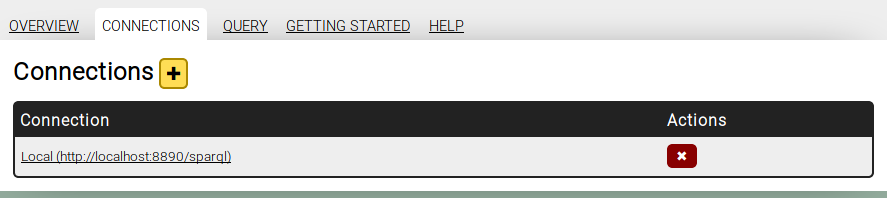
\includegraphics[width=1.0\textwidth]{figures/web-connections.png}
    \end{center}
    \caption{The \emph{connections} page enables users to configure accessible
      SPARQL endpoints.  Adding a connection here will provide an option to
      query it on the \emph{query} page.}
    \label{fig:web-connections}
  \end{figure}

\section{Managing projects}
\label{sec:web-projects}

  Projects are a loosely-defined way to group queries and to collaborate with
  other users.  Projects provide a way to manage access to \emph{graphs}, and
  to share previously-executed queries among project members.

  Marking a project as ``active'' indicates that queries executed using the web
  interface relate to that project.  See also section \ref{sec:query-history}
  {\color{LinkGray}`\nameref{sec:query-history}'}.

\section{Executing queries}

  After configuring at least one endpoint, it can be chosen on the \emph{query}
  page to execute a query against it.

  \begin{figure}[H]
    \begin{center}
      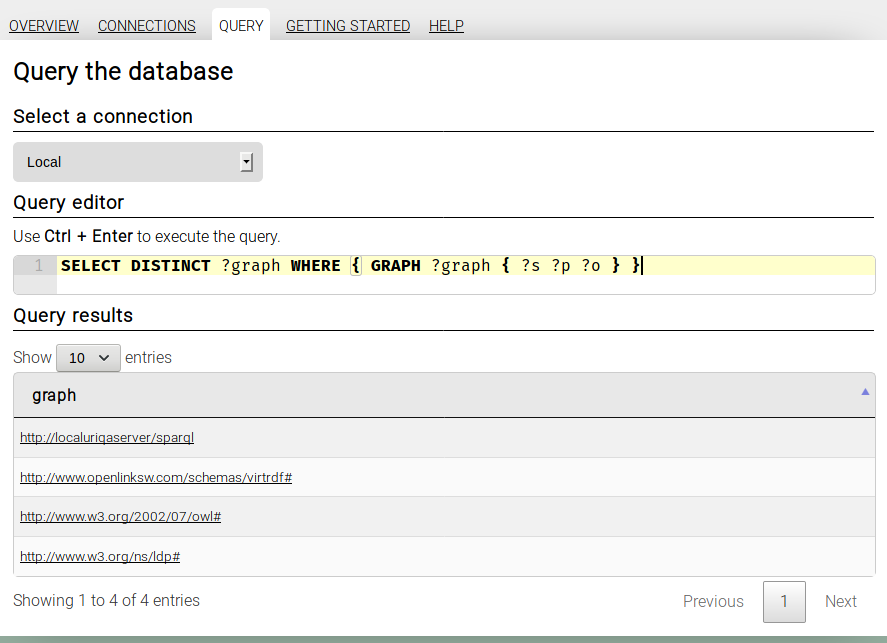
\includegraphics[width=1.0\textwidth]{figures/web-query.png}
    \end{center}
    \caption{The \emph{query} page enables users to execute a query against a
      SPARQL endpoint.  The connections configured at the \emph{connections} page
      can be chosen from the drop-down menu.}
    \label{fig:web-query}
  \end{figure}

\subsection{Query history}
\label{sec:query-history}

  When prototyping SPARQL queries, better known as ``SPARQLing around'', it's
  good to know that all queries that yielded a result are stored in the
  \emph{query history}.  The history is shown on the \emph{query} page below the
  query editor.

  Each \emph{project} has its own query history, and newly executed queries are
  added to the current \emph{active} project.

\section{Explore graphs with the Exploratory}

  Another utility aimed at SPARQLing around faster is the \emph{exploratory}.

  \begin{figure}[H]
    \begin{center}
      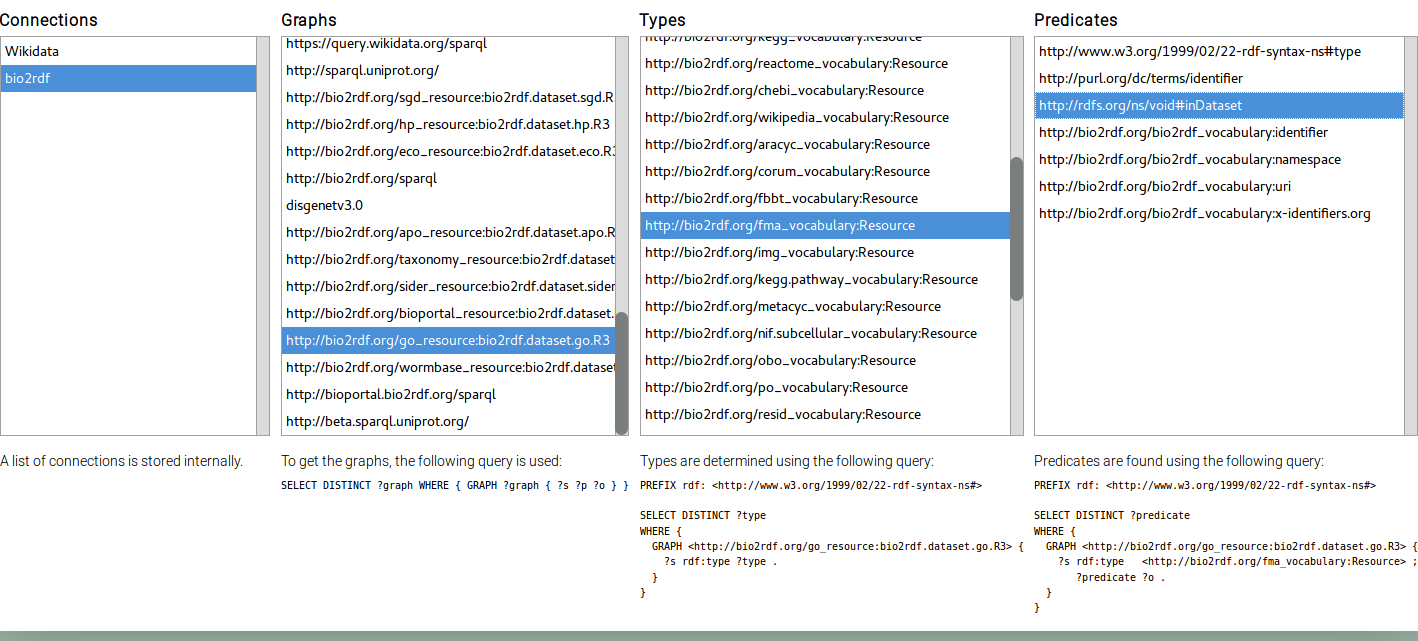
\includegraphics[width=1.0\textwidth]{figures/web-exploratory.png}
    \end{center}
    \caption{The \emph{exploratory} page enables users to learn about the
      structure of the triplets in a graph.}
    \label{fig:web-exploratory}
  \end{figure}

  The exploratory uses a common pattern in RDF to help writing queries.  Its
  interface provides a four-step selection process to find \emph{predicates}
  associated with an \texttt{rdf:type}.  The programs described in chapter
  \ref{chap:command-line} {\color{LinkGray}`\nameref{chap:command-line}'}
  automatically add the \texttt{rdf:type} annotations.

\subsection{Connections and graphs}

  The first step in finding predicates involves choosing a connection
  (see section \ref{sec:configure-connections} {\color{LinkGray}%
    `\nameref{sec:configure-connections}'}).  The second step involves
  choosing a graph.  If the connection does not support the use of graphs,
  the journey ends here.

\subsection{Types}

  The third step looks for triplets that match the pattern \emph{subject}
  $\rightarrow$ \texttt{rdf:type} $\rightarrow$ \emph{type}.  All matches for
  \emph{type} are displayed.  For data imported with \texttt{vcf2rdf} (see
  section \ref{sec:vcf2rdf} {\color{LinkGray}`\nameref{sec:vcf2rdf}'}), this
  will display (among other types) the \texttt{VariantCall} type.

\subsection{Predicates}

  Staying with the \texttt{VariantCall} example;  All data properties extracted
  from a VCF file can be found under this type.  A predicate displayed in this
  column occurs in \emph{at least} one triplet.  It not necessarily occurs in
  \emph{every} triplet.  Especially when using \texttt{INFO} and \texttt{FORMAT}
  fields in a VCF file, we recommend using them in a query inside an
  \texttt{OPTIONAL} clause.

\pagebreak{}
\section{Programming interface}
\label{sec:web-api}

  Other than a user interface, the web interface provides a programming interface
  using the HyperText Transport Protocol (HTTP).  The interface supports XML,
  JSON, and S-expressions.  Table \ref{table:api-return-formats} summarizes the
  supported formats.

  \hypersetup{urlcolor=black}
  \begin{table}[H]
    \begin{tabularx}{\textwidth}{l!{\VRule[-1pt]}X}
      \headrow
      \textbf{Content-Type} & \textbf{Example response}\\
      \evenrow
      \texttt{application/json}
      & \texttt{[\{ "message": "This is a JSON response." \}]}\\
      \oddrow
      \texttt{application/xml}
      & \texttt{<message>This is a XML response.</message>}\\
      \evenrow
      \texttt{application/s-expression}
      & \texttt{(message . "This is a S-expression response.")}\\
    \end{tabularx}
    \caption{\small Implemented content types for the API.  The
      \texttt{Content-Type} can be used in the \texttt{Accept} HTTP header.}
    \label{table:api-return-formats}
  \end{table}
  \hypersetup{urlcolor=LinkGray}

\subsection{Formatting \texttt{POST} requests}

  The \texttt{Accept} parameter influences the response format of the API,
  and the \texttt{Content-Type} parameter can be used to indicate the format
  of the request.

  In addition to the documented \texttt{Content-Type} values, the type
  \texttt{application/x-www-form-urlencoded} is also allowed, which expects
  the following format:
\begin{siderules}
\begin{verbatim}
parameter1=value1&parameter2=value2&...
\end{verbatim}
\end{siderules}

  The \texttt{Content-Type} header line does not have to be equal to the
  \texttt{Accept} header line, so for example, parameters can be sent in
  XML and the response can be formatted in JSON or the other way around.

\subsection{Conventions when using XML}

\begin{sloppypar}
  When using XML, there are a few conventions to follow.  To communicate a list
  or array of records, the API relies on using pre-defined elements. The API
  expects parameters to be wrapped in \texttt{<parameters>...</parameters>}
  elements.  So, to log in using an XML request, the following message will be
  accepted:
\end{sloppypar}

\begin{siderules}
\begin{verbatim}
POST /api/login HTTP/1.1
Host: ...
Content-Type: application/xml
Content-Length: 80
Connection: close

<parameters>
  <username>...</username>
  <password>...</password>
</parameters>
\end{verbatim}
\end{siderules}

  Subsequently, when \texttt{Accept}ing XML the results are wrapped in
  \texttt{<results>...</results>}, and data structures built from multiple
  key-value pairs are wrapped in \texttt{<result>...<result>}.  The
  following example illustrates receiving a project record:

\begin{siderules}
\begin{verbatim}
GET /api/projects HTTP/1.1
Host: ...
Accept: application/xml
Cookie: ...
Connection: close

<results>
  <result>
    <projectId>http://sparqling-genomics.org/0.99.10/Project/...</projectId>
    <creator>http://sparqling-genomics.org/0.99.10/Agent/...</creator>
    ...
  </result>
</results>
\end{verbatim}
\end{siderules}

\textbf{Note}: The actual response strips the whitespace.  It was added to
this example for improved readability.

\subsection{Authenticating API requests with \texttt{/api/login}}
\label{sec:api-login}

  Before being able to interact with the API, a session token must be obtained.
  This can be done by sending a \texttt{POST}-request to \texttt{/api/login},
  with the following parameters:

  \hypersetup{urlcolor=black}
  \begin{table}[H]
    \begin{tabularx}{\textwidth}{l!{\VRule[-1pt]}X!{\VRule[-1pt]}X}
      \headrow
      \textbf{Parameter} & \textbf{Example} & \textbf{Required?}\\
      \evenrow
      \texttt{username}  & \texttt{jdoe}   & Yes\\
      \oddrow
      \texttt{password}  & \texttt{secret} & Yes\\
    \end{tabularx}
  \end{table}
  \hypersetup{urlcolor=LinkGray}

  The following cURL command would log the user \texttt{jdoe} in:

\begin{siderules}
\begin{verbatim}
curl --cookie-jar - http://localhost/api/login \
     --data "username=jdoe&password=secret"
\end{verbatim}
\end{siderules}

  The response contains a cookie with the session token.  Use this cookie in
  subsequent requests.  When authentication fails, the service will respond
  with HTTP status-code \texttt{401}.

\subsection{Managing connections}

  The API can be used to store connections and refer to them by name.  The
  remainder of this section describes the API calls related to connections.

\subsubsection{Retrieve connections with \texttt{/api/connections}}

  With a call to \texttt{/api/connections}, the pre-configured connections
  can be viewed.  This resource expects a \texttt{GET} request and needs no
  parameters.  It returns all connection records associated with the currently
  logged-in user.

  The following cURL command would retrieve all connection records in JSON
  format:

\begin{siderules}
\begin{verbatim}
curl http://localhost/api/connections \
     --cookie "$COOKIE"               \
     -H "Accept: application/json"
\end{verbatim}
\end{siderules}

\subsubsection{Create a new connection with \texttt{/api/add-connection}}
\label{sec:api-create-connection}

  A call to \texttt{/api/add-connection} will create a new connection.
  The table below summarizes the parameters that can be used in this call.

  \hypersetup{urlcolor=black}
  \begin{table}[H]
    \begin{tabularx}{\textwidth}{l!{\VRule[-1pt]}X!{\VRule[-1pt]}X}
      \headrow
      \textbf{Parameter} & \textbf{Example} & \textbf{Required?}\\
      \evenrow
      \texttt{name}      & \texttt{Example}            & Yes\\
      \oddrow
      \texttt{uri}       & \texttt{http://my/endpoint} & Yes\\
      \evenrow
      \texttt{username}  & \texttt{jdoe}               & No\\
      \oddrow
      \texttt{password}  & \texttt{secret}             & No\\
      \evenrow
      \texttt{backend}   & \texttt{4store}             & No\\
    \end{tabularx}
  \end{table}
  \hypersetup{urlcolor=LinkGray}

  The following cURL command would create a connection, using JSON as
  the format to express the parameters:

\begin{siderules}
\begin{verbatim}
curl http://localhost/api/add-connection          \
     --cookie "$COOKIE"                           \
     -H "Accept: application/xml"                 \
     -H "Content-Type: application/json"          \
     --data '{ "name":     "Example",             \
                "uri":      "http://my/endpoint", \
                "username": "jdoe",               \
                "password": "secret",             \
                "backend":  "4store" }'
\end{verbatim}
\end{siderules}

\subsubsection{Remove a connection with \texttt{/api/remove-connection}}

  A call to \texttt{/api/remove-connection} will remove an existing
  connection.  The table below summarizes the parameters that can be
  used in this call.

  \hypersetup{urlcolor=black}
  \begin{table}[H]
    \begin{tabularx}{\textwidth}{l!{\VRule[-1pt]}X!{\VRule[-1pt]}X}
      \headrow
      \textbf{Parameter} & \textbf{Example} & \textbf{Required?}\\
      \evenrow
      \texttt{name}      & \texttt{Example} & Yes\\
    \end{tabularx}
  \end{table}
  \hypersetup{urlcolor=LinkGray}

  The following cURL command would remove the connection that was created in
  section \ref{sec:api-create-connection} {\color{LinkGray}`%
    \nameref{sec:api-create-connection}'}:

\begin{siderules}
\begin{verbatim}
curl http://localhost/api/remove-connection       \
     --cookie "$COOKIE"                           \
     -H "Accept: application/xml"                 \
     --data "name=Example"
\end{verbatim}
\end{siderules}

\subsection{Managing projects}

  The API has various resources to manage projects, as described in
  section \ref{sec:web-projects} {\color{LinkGray}`\nameref{sec:web-projects}'}.

\subsubsection{Retrieve a list of projects with \texttt{/api/projects}}

  Retrieving a list of projects can be done by sending a \texttt{GET} request
  to \texttt{/api/projects}.

  The following cURL command would retrieve a list of projects:

\begin{siderules}
\begin{verbatim}
curl http://localhost/api/projects      \
     --cookie "$COOKIE"                 \
     -H "Accept: application/xml"
\end{verbatim}
\end{siderules}

\subsubsection{Create a new project with \texttt{/api/add-project}}
\label{sec:api-add-project}

  To create a new project, send a \texttt{POST} request to
  \texttt{/api/add-project}.  The table below summarizes the parameters
  that can be used with this call.

  \hypersetup{urlcolor=black}
  \begin{table}[H]
    \begin{tabularx}{\textwidth}{l!{\VRule[-1pt]}X!{\VRule[-1pt]}X}
      \headrow
      \textbf{Parameter} & \textbf{Example} & \textbf{Required?}\\
      \evenrow
      \texttt{name}      & \texttt{Example project} & Yes\\
    \end{tabularx}
  \end{table}
  \hypersetup{urlcolor=LinkGray}

  The following cURL command would add a project:

\begin{siderules}
\begin{verbatim}
curl http://localhost/api/add-project      \
     --cookie "$COOKIE"                    \
     -H "Accept: application/xml"          \
     --data "name=Example project"
\end{verbatim}
\end{siderules}

\subsubsection{Remove a project with \texttt{/api/remove-project}}

  To remove a project, send a \texttt{POST} request to
  \texttt{/api/remove-project}.  The table below summarizes the parameters
  that can be used with this call.

  \hypersetup{urlcolor=black}
  \begin{table}[H]
    \begin{tabularx}{\textwidth}{l!{\VRule[-1pt]}l!{\VRule[-1pt]}X}
      \headrow
      \textbf{Parameter}   & \textbf{Example} & \textbf{Required?}\\
      \evenrow
      \texttt{project-uri}
      & \texttt{http://sparqling-genomics.org/Project/640c0...5a6d2} & Yes\\
    \end{tabularx}
  \end{table}
  \hypersetup{urlcolor=LinkGray}

  The following cURL command would remove the project created in
  \ref{sec:api-add-project} {\color{LinkGray}`%
    \nameref{sec:api-add-project}'}:

\begin{siderules}
\begin{verbatim}
curl http://localhost/api/remove-project      \
     --cookie "$COOKIE"                       \
     -H "Accept: application/xml"             \
     --data "project-uri=http://sparqling-genomics.org/Project/640c0...5a6d2"
\end{verbatim}
\end{siderules}

\subsubsection{Retrieve the active project with \texttt{/api/active-project}}

  This resource expects a \texttt{GET} request and needs no parameters.
  It returns a record of the current active project.

  The following cURL command retrieves the active project record as
  S-expression:

\begin{siderules}
\begin{verbatim}
curl http://localhost/api/active-project      \
     --cookie "$COOKIE"                       \
     -H "Accept: application/s-expression"
\end{verbatim}
\end{siderules}

\subsubsection{Make a project active with \texttt{/api/set-as-active-project}}

  The \texttt{/api/set-as-active-project} call can be used to change the
  ``active project''.  This resource expects a \texttt{POST} request with
  a \texttt{project-uri} as its parameter.  The \texttt{project-uri} can be
  obtained from a call to \texttt{/api/projects}.

  The following table summarizes the parameters that can be used with this call.

  \hypersetup{urlcolor=black}
  \begin{table}[H]
    \begin{tabularx}{\textwidth}{l!{\VRule[-1pt]}X!{\VRule[-1pt]}X}
      \headrow
      \textbf{Parameter}   & \textbf{Example} & \textbf{Required?}\\
      \evenrow
      \texttt{project-uri} & \texttt{http://example/project} & Yes\\
    \end{tabularx}
  \end{table}
  \hypersetup{urlcolor=LinkGray}

  The following cURL command changes the \emph{active project}:

\begin{siderules}
\begin{verbatim}
curl http://localhost/api/set-as-active-project \
     --cookie "$COOKIE"                         \
     -H "Accept: application/xml"               \
     --data "project-uri=${PROJECT_URI}"
\end{verbatim}
\end{siderules}

\subsubsection{Assign a graph to a project \texttt{/api/assign-graph}}

  Assigning a graph to a project can be done by sending a \texttt{POST} request
  to \texttt{/api/assign-graph}.  The required parameters are:

  \begin{itemize}
    \item{\texttt{project-uri}: This can be obtained from a call to
      \texttt{/api/projects}.}
    \item{\texttt{graph-uri}: The graph URI to assign.}
  \end{itemize}

  The following example based on cURL shows how to perform the request:
\begin{siderules}
\begin{verbatim}
curl -X POST                                               \
     -H "Accept: application/json"                         \
     -H "Content-Type: application/json"                   \
     --cookie "SGSession=..."                              \
     --data '{ "project-uri": "http://the-project-uri",    \
               "graph-uri": "http://the-new-graph-name" }' \
     http://localhost/api/assign-graph
\end{verbatim}
\end{siderules}

\subsubsection{Unassign a graph from a project with \texttt{/api/unassign-graph}}

  Like assigning a graph to a project, it can be unassigned as well using
  \texttt{/api/unassign-graph} using the same parameters as
  \texttt{/api/assign-graph}.

  The following example based on cURL shows how to perform the request:
\begin{siderules}
\begin{verbatim}
curl -X POST                                               \
     -H "Accept: application/json"                         \
     -H "Content-Type: application/json"                   \
     --cookie "SGSession=..."                              \
     --data '{ "project-uri": "http://the-project-uri",    \
               "graph-uri": "http://the-new-graph-name" }' \
     http://localhost/api/unassign-graph
\end{verbatim}
\end{siderules}

\subsection{Running and viewing queries}

\subsubsection{Retrieve previously run queries with \texttt{/api/queries}}

  When running queries through SPARQLing-genomics's interface, each succesful
  query is stored in a ``query history''.  This query history can be retrieved
  using a call to \texttt{/api/queries}.  This resource expects a \texttt{GET}
  request.

  The following cURL command would retrieve the entire query history, formatted
  as XML:

\begin{siderules}
\begin{verbatim}
curl http://localhost/api/queries \
     --cookie "$COOKIE"           \
     -H "Accept: application/xml"
\end{verbatim}
\end{siderules}
